%
% PSI Programmer's Manual
%
% SVN Revision Control Section
% (formerly CVS)
%
% TDC, February, 1996
% Modified by TDC, December 2002
% Updated from CVS to SVN, April 2007
%

The subversion control system (SVN) (\htmladdnormallink{{\tt
    subversion.tigris.org}}{http://subversion.tigris.org/}) provides a
convenient means by which programmers may obtain the latest (or any
previous) version of the \PSIthree\ source from the main repository or
a branch version, add new code to the source tree or modify existing
\PSIthree\ modules, and then make changes and additions available to
other programmers by checking the modifications back into the main
repository.  SVN also provides a ``safety net'' in that any erroneous
modifications to the code may be easily removed once they have been
identified.  This section describes how to use SVN to access and
modify the \PSIthree\ source code.  (Note that compilation and
installation instructions are given in a separate document.)

The main repository for the \PSIthree\ Source code is currently
maintained by the Crawford group at Virginia Tech.  To check out the
code, one must first obtain an SVN account by emailing
\htmladdnormallink{{\tt crawdad@vt.edu}}{mailto:crawdad@vt.edu}.
After you have a login-id and password, you are now ready to access
the repository via a secure, SSL-based WebDAV connection, but first
you must decide which version of the code you need.

The PSI3 SVN repository contains three top-level directories:
\begin{itemize}
\item {\tt trunk}: The main development area.
\item {\tt branches}: Release branches and private development
  branches are stored here.
\item {\tt tags:} Snapshots of the repository corresponding to public
  releases are stored here and should {\em never} be modified.
\end{itemize}
If you have a PSI3 SVN account, you can peruse these directories if
you like by pointing web browser to:

\noindent
{\tt https://sirius.chem.vt.edu/svn/psi3/}

\subsection{\PSIthree\ SVN Policies: Which Branch Should I Use?}
\label{section:branches}

The \PSIthree\ repository is comprised of a main trunk and several
release branches.  The branch you should use depends on the sort of 
work you plan for the codes:
\begin{enumerate}
\item For any piece of code already in the most recent release, bug
  fixes (defined as anything that doesn't add functionality ---
  including documentation updates) should be made {\em only} on the
  most recent stable release branch.
\item The main trunk is reserved for development of new functionality.
  This allows us to keep new, possibly unstable code away from public
  access until the code is ready.
\item Code that you do not want to put into next major release of
  \PSIthree\ should be put onto a separate branch off the main
  trunk. You will be solely responsible for maintenance of the new
  branch, so you should read the SVN manual before attempting this.
\end{enumerate}

\noindent Fig.~\ref{Fig:svn} provides a schematic of the SVN
revision-control structure and branch labeling.  Two release branches
are shown, the current stable branch, named {\tt psi-3-3}, and a
planned future release, to be named {\tt psi-3-4}.  The tags on the
branches indicate release points, where bugs have been fixed and the
code has been or will be exported for public distribution.  As soon as
a release branch is created, we generate a tag so that we may make
updates to that version of the code without affecting other branches
or the main trunk.  The dotted lines in the figure indicate merge
points: before each public release, changes made to the code on the
stable release branch will be merged into the main trunk.

% We have adopted the convention that the first tag on a new release
% branch will be given the suffix, {\tt -rc-1}, for ``release candidate
% 1'' (i.e., a numbered beta release).  Subsequent tags for new released
% on the same branch will be updated with {\tt -rc-2}, {\tt -rc-3}, etc.
% Once the code is appropriately stable to be beyond beta status,
% release tags will be given the suffix, {\tt -0}, {\tt -1}, etc.,
% indicating patch levels.  


\begin{figure}[h]
\begin{center}
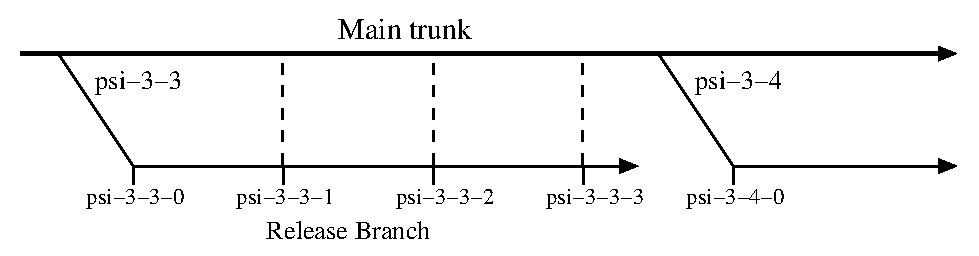
\epsfig{file=svn.eps,height=3.5cm}
\end{center}
\caption{\PSIthree\ SVN branch structure with examples of branch- and
release-tag labelling.}
\label{Fig:svn}
\end{figure}

\noindent A frequently encountered problem is what to do about bug fixes
that are necessary for uninterrupted code development of the code on the
main trunk. As Rule 1 of the above policy states, all bug fixes of the code
already in the recent stable release must go on the corresponding branch,
not on the main trunk. The next step depends on the severity of the bug:
\begin{enumerate}
\item If the bug fix is critical and potentially affects every
  developer of the code on the main trunk, then \PSIthree\
  administrators should be notified of the fix. If deemed necessary,
  appropriate steps to create a new patch release will be made. Once
  the next patch release is created then the bug fixes will be merged
  onto the main trunk.  If the bug fix doesn't warrant an immediate
  new patch release, then you can incorporate the bug fix into your
  local copy of the main trunk code manually or using SVN merge
  features. This will allow you to continue development until next
  patch release is created and the bug fix is incorporated into the
  main trunk code in the repository. However you should {\em never}
  merge such changes into the main trunk yourself.
\item If the bug fix is not critical (e.g. a documentation
  update/fix), then you should wait until next patch release when it
  will be merged into the main trunk automatically.
\end{enumerate}

\noindent
The following are some of the most commonly used SVN commands for checking
out and updating working copies of the \PSIthree\ source code.

\noindent
$\bullet$ To checkout a working copy of the head of the main trunk:

{\tt svn co https://sirius.chem.vt.edu/svn/psi3/trunk/ psi3} 

\noindent
$\bullet$ To check out a working copy of the head of a specific release branch,
e.g., the branch labelled {\tt psi-3-3}:

{\tt svn co https://sirius.chem.vt.edu/svn/psi3/branches/psi-3-3 psi3}

\noindent Note that subsequent {\tt svn update} commands in this
working copy will provide updates only on the chosen branch.  Note
also that after you have checked out a fresh working copy of the code
you must run the {\tt autoconf} command to generate a {\tt configure}
script for building the code.  (See the installation manual for
configuration, compilation, and testing instructions.)

\noindent For each of the above commands, the working copy of your
code will be placed in the directory \file{psi3}, regardless of your
choice of branch.  In this manual, we will refer to this directory
from now on as {\tt \$PSI3}.  Subsequent SVN commands are usually run
within this top-level directory.

\noindent
$\bullet$ To update your current working copy to include the latest revisions:

{\tt svn update}

\noindent
Notes: (a) This will update only the revisions on your current branch;
(b) The old {\tt -d} and {\tt -P} flags required by CVS are not necessary with SVN. 

\noindent
$\bullet$ To convert your working copy to the head of a specific branch:

{\tt svn switch https://sirius.chem.vt.edu/svn/psi3/branches/psi-3-3}

\noindent
$\bullet$ To convert your working copy to the head of the main trunk:

{\tt svn switch https://sirius.chem.vt.edu/svn/psi3/trunk/}

\noindent
$\bullet$ To find out what branch your working copy is on, run this in your
top-level \PSIthree\ source directory:

{\tt svn info | grep URL}

\noindent
This will return the SVN directory from which your working copy was
taken, e.g.,

\noindent
{\tt URL: https://sirius.chem.vt.edu/svn/psi3/branches/psi-3-3}

\noindent
Some words of advice:
\begin{enumerate}
\item Most SVN commands are reasonably safe, 

\item Unlike CVS, you shouldn't use {\tt svn update} to see the status
  of your working copy.  With SVN you should use {\tt svn status} to
  see if you've modified any files or directories.  If you want a
  direct comparison with the repository, you should use {\tt svn status -u}.
\item Read the SVN manual.  Seriously.
\begin{center}
\htmladdnormallink{{\tt
http://svnbook.red-bean.com/en/1.2/svn-book.html}}{http://svnbook.red-bean.com/en/1.2/svn-book.html}
\end{center}
\item If you're about to start some significant development or bug-fixes,
first update your working copy to the latest version on your branch.
In addition, if you do development over a long period of time (say weeks to
months) on a specific module or modules, be sure to run a {\tt svn status -u}
occasionally. In can be {\em very} frustrating to try to check in lots
of changes, only to find out that the \PSIthree\ has changed dramatically
since your last update.
\end{enumerate}

\subsection{Checking in altered \PSIthree\ binaries or libraries}

If you have changes to Psi binaries or libraries which already exist, one
of two series of steps is necessary to check these changes in to the main
repository. The first series may be followed if all changes have been made
only to files which already exist in the current version. The second series
should be followed if new files must be added to the code in the repository.

\begin{itemize}
\item No new files need to be added to the repository. We will use
\library{libciomr} as an example. 
\begin{enumerate}
\item {\tt cd \$PSI3/src/lib/libciomr}
\item {\tt svn ci -m ``Put comments here.''}
\end{enumerate}
\item New files must be added to the repository. Again, we use 
\library{libciomr}
as an example. Suppose the new file is named \file{great\_code.c} .
\begin{enumerate}
\item {\tt cd \$PSI3/src/lib/libciomr} 
\item {\tt svn add great\_code.c} 
\item {\tt svn ci -m ``Put comments here.''}
\end{enumerate}
\end{itemize}

The \file{svn ci} command in both of these sequences will examine all
of the code in the current \file{libciomr} directory against the
current version of the code in the main repository. Any files which
have been altered (and for which no conflicts with newer versions
exist!) will be identified and checked in to the main repository (as
well as the new file in the second situation).

SVN requires that you include a comment on your changes.  However,
unlike CVS, SVN prefers that you put your comments on the command-line
rather than editing a text file.  I prefer the CVS way, but this is a
minor pain compared to all the advantages of SVN, in my opinion.

\subsection{Adding entirely new code to the main \PSIthree\ repository} 
\label{checkin_new}

If the programmer is adding a new executable module or library to the
\PSIthree\ repository, a number of important conventions should be followed:

\begin{enumerate}
\item Since such changes almost always involve additional functionality,
new modules or libraries should be added only on the main SVN trunk.
See section \ref{section:branches} for additional information.

\item The directory containing the new code should be given a name
  that matches the name of the installed code (e.g. if the code will
  be installed as \module{newcode}, the directory containing the code
  should be named \file{newcode}). New executable modules must be
  placed in \shellvar{\$PSI3}\file{/src/bin} and libraries in
  \shellvar{\$PSI3}\file{/src/lib} of the user's working copy.

\item The Makefile should be converted to an input file for the
  configure script (\file{Makefile.in} --- see any of the current
  \PSIthree\ binaries for an example) and should follow the
  conventions set up in all of the current \PSIthree\
  \file{Makefiles}. This includes use of \file{MakeVars} and
  \file{MakeRules}.

\item New binaries should be added to the list contained in
  \shellvar{\$PSI3}\file{/src/bin/Makefile.in} so that they will be
  compiled automatically when a full compilation of the \PSIthree\
  distribution occurs. This step is included in the sequence below.

\item A documentation page should be included with the new code (see
  section \ref{Documentation} for more information). As a general
  rule, if the code is not ready to have a documentation page, it is
  not ready to be installed in \PSIthree.

\item The \file{configure.ac} file must be altered so that users may
  check out copies of the new code and so that the \file{configure}
  script will know to create the Makefile for the new code. These
  steps are included in the sequence below.

\end{enumerate}

Assume the new code is an executable module and is named
\module{great\_code}. The directory containing the new code must
contain only those files which are to be checked in to the repository!
Then the following steps will check in a new piece of code to the main
repository:

\begin{enumerate}
\item {\tt cd \$PSI3/src/bin}
\item {\tt svn add great\_code}
\item {\tt svn ci -m ``Put comments here.''}
\item {\tt cd \$PSI3}
\item Edit \file{configure.ac} and add \file{great\_code} to the list. 
\item {\tt svn ci configure.ac -m ``Put comments here.''}
\item {\tt autoconf} 
\item {\tt cd \$PSI3/src/bin} 
\item Edit \file{Makefile.in} and add \file{great\_code} to the list. 
\item {\tt svn ci Makefile.in -m ``Put comments here.''}
\end{enumerate}
At this point, all of the code has been properly checked in, but you
should also test to make sure that the code can be checked out by
other programmers, and that it will compile correctly. The following
steps will store your personal version of the code, check out the new
code, and test-compile it:
\begin{enumerate}
\item {\tt cd \$PSI3/src/bin}
\item {\tt mv great\_code great\_code.bak}
\item {\tt cd \$PSI3/..}
\item {\tt svn update}
\item {\tt cd \$objdir}
\item {\tt \$PSI3/configure -}{\tt -prefix=\$prefix}
\item {\tt cd src/bin/great\_code}
\item {\tt make install}
\end{enumerate}
(Note that \$prefix and \$objdir to the installation and compilation
 directories defined in the \PSIthree\ installation instructions.)
Your original version of the code remains under \file{great\_code.bak},
but should be no longer necessary if the above steps work. Note that it is
necessary to re-run \file{configure} explicitly, instead of just running
\file{config.status}, because the latter contains no information about
the new code.

\subsection{Updating checked out code}

If the code in the main repository has been altered, other users' working
copies will of course not automatically be updated.  In general, it is
only necessary to execute the following steps in order to completely update
your working copy of the code:

\begin{enumerate}
\item {\tt cd \$PSI3}
\item {\tt svn update}
\end{enumerate}

This will examine each entry in your working copy and compare it to
the most recent version in the main repository. When the file in the
main repository is more recent, your version of the code will be
updated. If you have made changes to your version, but the version in
the main repository has not changed, the altered code will be
identified to you with an ``M''. If you have made changes to your
version of the code, and one or more newer versions have been updated
in the main repository, SVN will examine the two versions and attempt
to merge them -- this process often reveals conflicts, however, and is
sometimes unsuccessful. You will be notified of any conflicts that
arise (labelled with a ``C'') and you must resolve them manually.

If new directories have been added to the repository, the update above
will automatically add them to your working copy.  However, you may
need to re-run {\tt autoconf} and configure ({\tt
  \$objdir/config.status --recheck} is a convenient command) to be
able to build the new code.

\subsection{Removing code from the repository}
If alterations of libraries or binaries under Psi involves the deletion of 
source code files from the code, these must be explicitly removed through SVN.

The following steps will remove a source code file named \file{bad\_code.F} 
from a binary module named \module{great\_code}:
\begin{enumerate}
\item {\tt cd \$PSI3/src/bin/great\_code}
\item {\tt svn remove bad\_code.F}
\item {\tt svn ci -m ``Put comments here.''}
\end{enumerate}

\subsection{Checking out older versions of the code}
It is sometimes necessary to check out older versions of a piece of code.
Assume we wish to check out an old version of \PSIdetci. If this
is the case, the following steps will do this:
\begin{enumerate}
\item {\tt cd \$PSI3/src/bin/detci}
\item {\tt svn co --revision \{2002-02-17\}}
\end{enumerate}

This will check the main repository and provide you with the code as
it stood exactly on February 17th, 2002. 

\subsection{Examining the revision history}
It can be very useful to use cvs to see what recent changes have been
made to the code.  Anytime one checks in a new version of a file, SVN
requires the user to provide comments on the changes with the {\tt -m}
flag.  These comments go into a log information that may be easily
accessed through SVN.  To see what changes have been made recently to
the file \file{detci.cc}, one would go into the \file{detci} source
directory and type
\begin{verbatim}
svn log detci.cc
\end{verbatim}
Checking the log files is a very useful way to see what recent changes might 
be causing new problems with the code.

\subsection{The structure of the \PSIthree\ Source Tree}
\label{psitree} 

Your working copy of the \PSIthree\ source code includes a number of
important subdirectories:

\begin{itemize}
\item \shellvar{\$PSI3}\file{/lib} -- Source files for
  OS-independent ``library'' data.  This includes the main basis set
  data file (\file{pbasis.dat}) and the \PSIthree\ program execution
  control file (\file{psi.dat}), among others.  These files are
  installed in \file{\$prefix/share}.

\item \shellvar{\$PSI3}\file{/include} -- Source files for
  OS-independent header files, including \file{physconst.h} (whose
  contents should be obvious from its name), \file{psifiles.h}, and
  \file{ccfiles.h}, among others.  These files are installed in
  \$prefix/include.

\item \shellvar{\$PSI3}\file{/src/util} -- Source code for the utility
  program \module{tocprint}.  (Note that the \module{tmpl} module is
  no longer used and will eventually disappear.)

\item \shellvar{\$PSI3}\file{/src/lib} -- Source code for the
  libraries, including \library{libpsio}, \library{libipv1},
  \library{libchkpt}, etc.  The include files from the library
  source are used directly during the compilation of PSI to 
  avoid problems associated with incomplete installations.  Some
  include files are architecture-dependent and go in an include
  subdirectory of the compilation (object) directory.

\item \shellvar{\$PSI3}\file{/src/bin} -- Source code for the
  executable modules.
\end{itemize}

After compilation and installation, the \file{\$prefix} directory
contains the executable codes and other necessary files.  {\bf NB:}
The files in this area should never be directly modified; rather, the
working copy should be modified and the \PSIthree\ \file{Makefile}
hierarchy should handle installation of any changes.  The structure of
the installation area is:

\begin{itemize}
\item \file{\$prefix/bin} -- The main executable directory.  This
  directory must be in your path in order for the driver program,
  \module{psi3}, to find the modules.

\item \file{\$prefix/lib} -- The \PSIthree\ code libraries.  (NB: The
  description of \PSIthree\ \file{Makefiles} later in this manual will
  explain how to use the libraries.)

\item \file{\$prefix/include} -- Header files.  These are not actually
  used during the compilation of PSI but are useful for inclusion by
  external programs because they are all in the same directory.

\item \file{\$prefix/share} -- OS-independent data files, including
  basis set information.  (Do not edit this file directly; any changes
  you make can be overwritten by subsequent {\tt make} commands.)

\item \file{\$prefix/doc} -- \PSIthree\ documentation, including
  installation, programmer, and user manuals.
\end{itemize}

